

\chapter{Bausteinsicht}

Um ein besseres Verständnis über die Struktur des Systems zu bekommen, nutzen wir die Bausteinsicht. Sie hilft dabei ein gemeinsames Verständnis des Systems innerhalb des Teams zu bekommen.
Die zur Zerlegung benutzte Dekompistionsstrategie ist funktional. 

\section{Bausteinsicht Level 1}
 

\begin{figure}[ht] % [h] = here
    \centering
    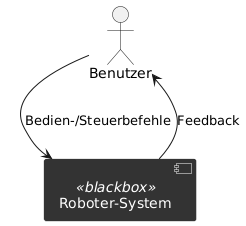
\includegraphics[width=0.6\textwidth]{diagrams/baustein_lvl_1_updated.png}
    \caption{Bausteinsicht Level 1}
\end{figure}

\begin{table}[h!]
\centering
\begin{tabular}{|p{4cm}|p{9cm}|}
\hline
\textbf{Komponente} & \textbf{Beschreibung} \\ \hline
Roboter-System & Gesamtsystem, das alle internen Steuer-, Safety- und Kommunikations­funktionen kapselt. Empfängt Bedien-/Steuerbefehle vom Benutzer, verarbeitet sie und liefert Feedback. \\ \hline
\end{tabular}
\caption{Bausteinsicht Level 1}
\label{tab:lvl1}
\end{table}

\newpage
\section{Bausteinsicht Level 2}
\begin{figure}[h] % [h] = here
    \centering
    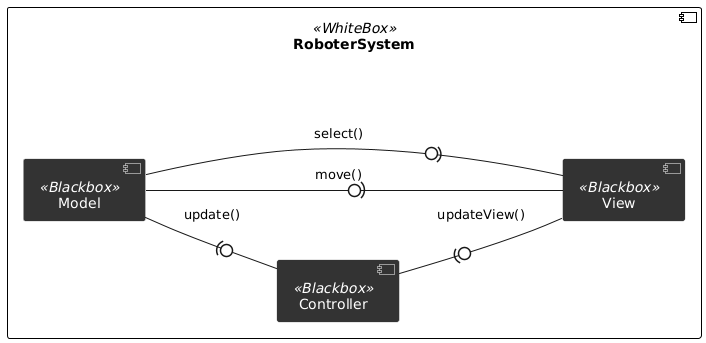
\includegraphics[width=0.6\textwidth]{diagrams/baustein_lvl_2_updated.png}
    \caption{Bausteinsicht Level 2}
\end{figure}

\begin{table}[h!]
\centering
\begin{tabular}{|p{4cm}|p{9cm}|}
\hline
\textbf{Komponente} & \textbf{Beschreibung} \\ \hline
Model & Beinhaltet die Geschäftslogik. Sendet Zustandsänderungen an den Controller. \\ \hline
Controller & Der Controller fungiert als Observer vom Model und gibt Zustandsänderungen des Models an die View weiter. \\ \hline
View & Bietet Interaktionsmöglichkeiten für den Nutzer und stellt dem Benutzer Informationen dar. 
\end{tabular}
\caption{Bausteinsicht Level 2}
\label{tab:lvl2}
\end{table}
\newpage

\section{Bausteinsicht Level 3 Model}
\begin{figure}[h] % [h] = here
    \centering
    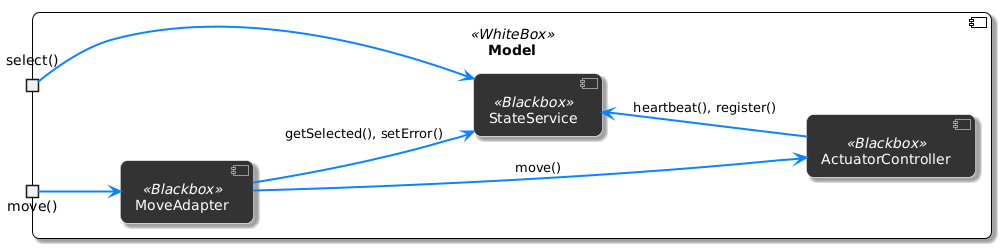
\includegraphics[width=0.6\textwidth]{diagrams/baustein_lvl_3_model.png}
    \caption{Bausteinsicht Level 3 Model}
\end{figure}

\begin{table}[h!]
\centering
\begin{tabular}{|p{4cm}|p{9cm}|}
\hline
\textbf{Komponente} & \textbf{Beschreibung} \\ \hline
StateService & Speichert den ausgewählten Roboter und die verfügbaren Roboter. Bei Zustandsänderungen informiert er den Controller. \\ \hline
MoveAdapter  & Empfängt einen Steuerungsbefehl vom View, übersetzt diesen mithilfe des StateServices, um den passenden Aktuator anzusprechen. \\ \hline
ActuatorController & Empfängt einen Steuerwert, überprüft die Gültigkeit und setzt diesen mithilfe der ICadsRoboticArm API. \\ \hline
\end{tabular}
\caption{Bausteinsicht Level 3}
\label{tab:lvl3}
\end{table}

\section{Bausteinsicht Level 3 View}
\begin{figure}[h] % [h] = here
    \centering
    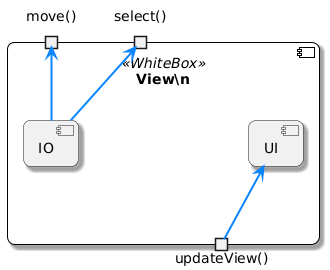
\includegraphics[width=0.6\textwidth]{diagrams/baustein_lvl_3_view.png}
    \caption{Bausteinsicht Level 3 View}
\end{figure}

\begin{table}[h!]
\centering
\begin{tabular}{|p{4cm}|p{9cm}|}
\hline
\textbf{Komponente} & \textbf{Beschreibung} \\ \hline
IO & Leitet die Eimgaben des Benutzers an den MoveAdapter weiter. \\ \hline
UI  & Stellt dem Nutzer dar welche Roboter verfügbar sind, welcher ausgewählt ist und informiert über Fehler.\\ \hline
\end{tabular}
\caption{Bausteinsicht Level 3}
\label{tab:lvl3}
\end{table}
